\documentclass[a4paper]{report}
\usepackage{float}
\usepackage{verbatim}
\usepackage[utf8]{inputenc}
\usepackage[italian]{babel}
\usepackage{amsmath, amsbsy,amssymb,amsfonts, amsthm, mhchem, multicol}
\usepackage{graphicx}
\usepackage[left=2cm,right=2cm,top=2cm,bottom=2cm]{geometry}
\usepackage{xcolor}
\usepackage[hypertexnames=false]{hyperref}
\usepackage{nameref}
\usepackage{framed}
\usepackage[framemethod=TikZ]{mdframed}

% figure support
\usepackage{import}
\usepackage{xifthen}
\pdfminorversion=7
\usepackage{pdfpages}
\usepackage{transparent}
\newcommand{\incfig}[1]{%
	\def\svgwidth{\columnwidth}
	\import{./figures/}{#1.pdf_tex}
}
\newcommand{\angstrom}{\mbox{\normalfont\AA}}
\newcommand{\bs}{\boldsymbol}

% title setup
\usepackage{xifthen}
\makeatother
\def\@lez{}%
\newcommand{\lez}[3]{
    \ifthenelse{\isempty{#3}}{%
        \def\@lez{Lezione #1}%
    }{%
        \def\@lez{Lezione #1: #3}%
    }%
    \section{\@lez}
    \marginpar{\small\textsf{\mbox{#2}}}
}
\makeatletter

%fatto
\newcounter{fact}[section]\setcounter{fact}{0}
\renewcommand{\thefact}{\arabic{section}.\arabic{fact}}
\newenvironment{fact}[2][]{%
\refstepcounter{fact}%
\ifstrempty{#1}%
{\mdfsetup{%
frametitle={%
\tikz[baseline=(current bounding box.east),outer sep=0pt]
\node[anchor=east,rectangle,fill=blue!20]
{\strut Fatto~\thefact};}}
}%
{\mdfsetup{%
frametitle={%
\tikz[baseline=(current bounding box.east),outer sep=0pt]
\node[anchor=east,rectangle,fill=blue!20]
{\strut Fatto~\thefact:~#1};}}%
}%
\mdfsetup{innertopmargin=10pt,linecolor=blue!20,%
linewidth=2pt,topline=true,%
frametitleaboveskip=\dimexpr-\ht\strutbox\relax
}
\begin{mdframed}[]\relax%
\label{#2}}{\end{mdframed}}

%definizione
\newcounter{defn}[section]\setcounter{defn}{0}
\renewcommand{\thedefn}{\arabic{section}.\arabic{defn}}
\newenvironment{defn}[2][]{%
\refstepcounter{defn}%
\ifstrempty{#1}%
{\mdfsetup{%
frametitle={%
\tikz[baseline=(current bounding box.east),outer sep=0pt]
\node[anchor=east,rectangle,fill=green!20]
{\strut Definizione~\thedefn};}}
}%
{\mdfsetup{%
frametitle={%
\tikz[baseline=(current bounding box.east),outer sep=0pt]
\node[anchor=east,rectangle,fill=green!20]
{\strut Definizione~\thedefn:~#1};}}%
}%
\mdfsetup{innertopmargin=10pt,linecolor=green!20,%
linewidth=2pt,topline=true,%
frametitleaboveskip=\dimexpr-\ht\strutbox\relax
}
\begin{mdframed}[]\relax%
\label{#2}}{\end{mdframed}}


\author{Edoardo Gabrielli}
\title{Appunti di astrofisica}

\begin{document}
\maketitle
\clearpage
\tableofcontents
%\clearpage
\chapter{Introduzione e Trasporto Radiativo}
\lez{1}{20-02-2020}{}
\subsubsection{Introduzione}%
Il corso è di astrofisica generale e darà una infarinatura generale degli argomenti principali dell'astrofisica.
\paragraph{Libro di testo}%
\texttt{Astrophysics for Physicists, Arnab Rai Choudhri}
\paragraph{Argomenti del corso}%
\begin{itemize}
	\item Trasporto radiativo.
	\item Stelle.
	\item Aggregati di stelle.
	\item Mezzo interstellare.
	\item Ammassi di galassie.
\end{itemize}
\subsection{Osservazione del cielo}%
\paragraph{Astrofisica}%
L'astrofisica è una scienza osservativa: non possiamo decidere di modificare il nostro "apparato", possiamo solo soltanto raccogliere informazioni attraverso le tecnologie di osservazione che abbiamo.\\
Le informazioni possono essere raccolte attraverso i diversi tipi di \textbf{messaggeri} che ci arrivano dal cosmo.\\
Il messaggero principale è la radiazione elettromagnetica, ultimamente si sono aggiunti altri portatori di informazioni: prima le particelle (neutrini) e successivamente le onde gravitazionali.\\ 
Resta il fatto che la stragrande maggioranza di informazioni che sappiamo dall'universo proviene dalla radiazione elettromagnetica.\\ 
Non potendo decidere quando i fenomeni avvengono sarà necessario sviluppare delle strategie che permettano di avere una sorta di \texttt{ridondanza osservativa} per riuscire ad accertare un supposto evento.

\paragraph{Osservazione della radiazione elettromagnetica}%
Fino all seconda guerra mondiale si osservava soltanto nella fascia dello spettro del visibile: tra i 4000 ed i 7000 \AA.\\
Successivamente, grazie all'invenzione del radar si sono aperte le regioni del Radio, X, Infrarosso, Gamma. Oggi si fanno osservazioni in tutto lo spettro. 

\paragraph{Lotta contro l'oscurità}%
La sfida è sempre stata nel vedere sorgenti deboli. Una sorgente può essere debole perchè è intrinsecamente debole (nana bianca antichissima, pianeti) oppure sorgenti intrinsecamente molto luminosi ma molto molto lontani. \\
Poter osservare oggetti sempre più lontani significa aumentare il numero di osservazione: posso avere più possibilità di osservare fenomeni mai visti prima e fare nuova fisica.\\
Per vedere oggetti sempre meno luminosi abbiamo bisogno di lenti dei telescopi sempre più grandi. Attualmente i telescopi ottici più grandi hanno diametri di 10 metri. L'ESA sta costruendo un telescopio di diametro di 39 metri. Avere un diametro più grande significa avere una sensibilità maggiore.

\subsection{Diffrazione e Seeing}%
\paragraph{Telescopi sempre più grandi}%
Aumentando la superficie della lente del telescopio aumenta la capacità di catturare luce e quindi la sensibilità del telescopio. Tuttavia questo non è l'unico motivo per cui si costruiscono telescopi sempre più grandi: c'è anche un motivo legato alla risoluzione del telescopio.\\
Quando guardiamo il cielo noi osserviamo degli angoli, le varie sorgenti che sono proiettate sulla volta celeste. La risoluzione è l'angolo più piccolo tra due sorgenti proiettate sulla volta celeste che mi permette di distinguerle.\\
Infatti per le dimensioni angolari degli oggetti luminosi nel cielo non sono trascurabili effetti di diffrazione. 
\paragraph{Diffrazione}%
Prendiamo il classico problema della fenditura:
\begin{figure}[H]
    \centering
    \incfig{diffrazione-da-una-fenditura}
    \caption{Diffrazione da una fenditura}
    \label{fig:diffrazione-da-una-fenditura}
\end{figure}
\noindent
Sappiamo che gli zeri della funzione di intensità $\frac{I}{I_0}$ sono nei punti:
\[
	\sin\theta = \frac{\lambda}{D}\cdot m \quad \quad m \text{ intero}
.\] 
Con il nostro telescopio abbiamo una situazione simile: abbiamo una stella lontana che irraggia. La sua luce entra in una fenditura circolare di diametro D data dal telescopio. Per il principio di Babinet sappiamo che anche in questo caso si crea una figura di interferenza che prenderà la seguente forma:
\begin{figure}[H]
	\centering
	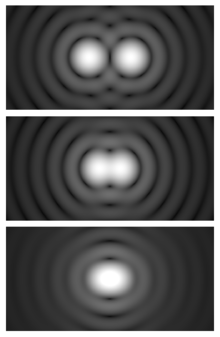
\includegraphics[width=0.2\textwidth]{figures/diffraction.png}
	\caption{\scriptsize Diffrazione al telescopio per due stelle al variare della risoluzione angolare.}
	\label{fig:diffraction}
\end{figure}
\noindent
Questa struttura di rifrazione ci permette di ridefinire il concetto di risoluzione, questa volta gli zeri sono in corrispondenza di alcuni numeri, il primo zero va ha $m=1.22$. \\
Il cerchio centrale, detto disco di Airy è importante perchè ci permette di discriminare due oggetti, questo risulta evidente in \hyperref[fig:diffraction]{Figura 2}\\
Prendendo angoli progressivamente più piccoli le figure di diffrazione tengono a sovrapporsi, il criterio per dire quando due sorgenti sono distinguibili è detto Criterio di Rayleigh: due sorgenti si dicono distinte quando hanno dischi di Hairy con centri che giacciono uno all'esterno dell'altro.
Quindi l'angolo minimo che riesco a risolvere sarà: 
\[
	\sin\theta_{min} \approx \theta_{min} =  1.22 \frac{\lambda}{D}
.\]
Quindi la risoluzione angolare di questo telescopio è data da questa formula. Per questo possiamo capire perchè è importante avere telescopi sempre più grandi.\\

Quando un telescopio arriva alla situazione in cui il limite di funzionamento è quello di diffrazione si dice che siamo nelle condizioni ottimali: quelle di Diffraction Limited (Hubble è in queste condizioni). 
\paragraph{Seeing}%
Sulla terra si può arrivare alla condizione ottimale del paragrafo precedente? In genere no per colpa della atmosfera, avente indice di diffrazione variabile è la maggiore fonte di disturbo.
\begin{figure}[H]
	\centering
	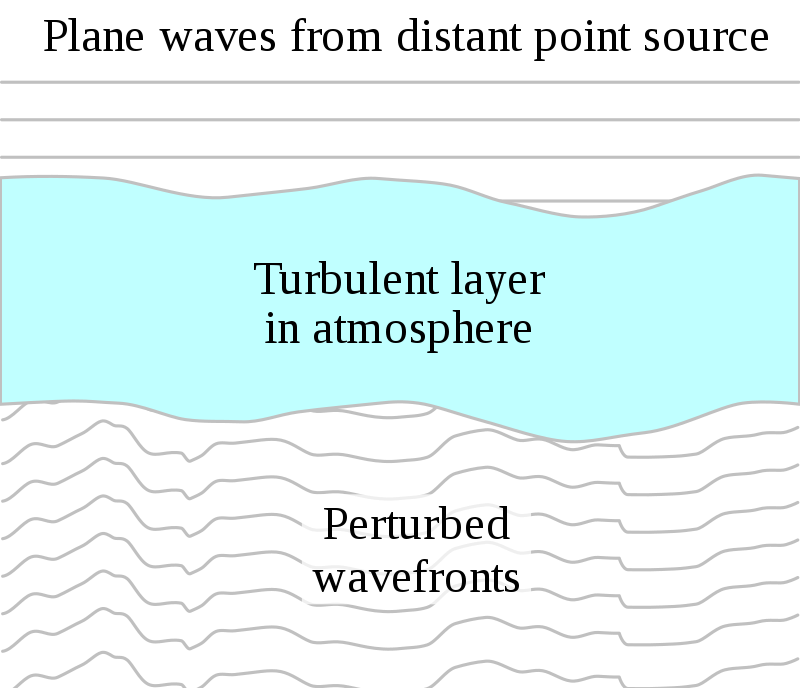
\includegraphics[width=0.3\textwidth]{figures/seeing.png}
	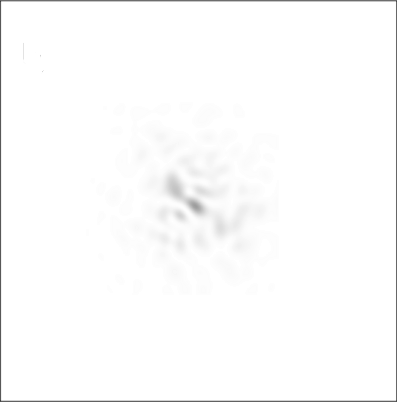
\includegraphics[width=0.2\textwidth]{figures/seeing-effect.png}
	\caption{\scriptsize A destra un possibile effetto sui fronti d'onda che attraversano l'atmosfera e a sinistra il risultato sulla stella agli occhi del telescopio, l'immagine risulta allargata e distorta.}
	\label{fig:figures-seeing-png}
\end{figure}
\noindent
Qual'è l'ordine di grandezza del Seeing? Se è buono si arriva al "secondo d'arco": $1''$. Nei siti migliori si arriva a $0.5''$.\\
Possiamo allora chiederci qual'è il valore del diametro del telescopio che mi produce un angolo di diffrazione minimo che corrisponde a quello del seeing. A quel punto non mi servirebbe a niente aumentare le dimensioni della lente: il seeing ci sarebbe comunque.\\
Nella luce visibile si ha $\lambda \approx 5000$ \AA, se prendiamo a questa lunghezza d'onda un angolo di $1''$ vediamo che il telescopio che raggiunge il limite del seeing è minuscolo: $D=$ 12 cm.\\
Perchè allora si costruiscono telescopi di 40 metri di diametro?
\begin{itemize}
	\item Per raccogliere comunque più luce.
	\item Per via dell'avvento della elettronica.
\end{itemize}
Esiste infatti un sistema detto ottica adattiva per correggere la presenza dell'atmosfera: si spara una sorgente laser in aria e si cercano di compensare elettronicamente l'effetto dell'atmosfera.
\paragraph{Lunghezza d'onda per cui oggi si ha la massima risoluzione angolare}%
Ha senso diminuire $\lambda$ fissando $D$, sembrerebbe quindi sensato andare nel Gamma, oggi invece si ha la risoluzione massima nel Radio grazie a Tecniche di interferometria: possiamo costruire array di telescopi che lavorano simultaneamente (si registra con orologi atomici l'arrivo del segnale): si arriva a  $D = 8600$ km (baseline molto lunga). Con questo metodo si arriva a risoluzioni di decine di micro arcosecondi! Questo è sicuramente il caso della foto del buco nero (30 arcosecondi). 
\begin{figure}[H]
	\centering
	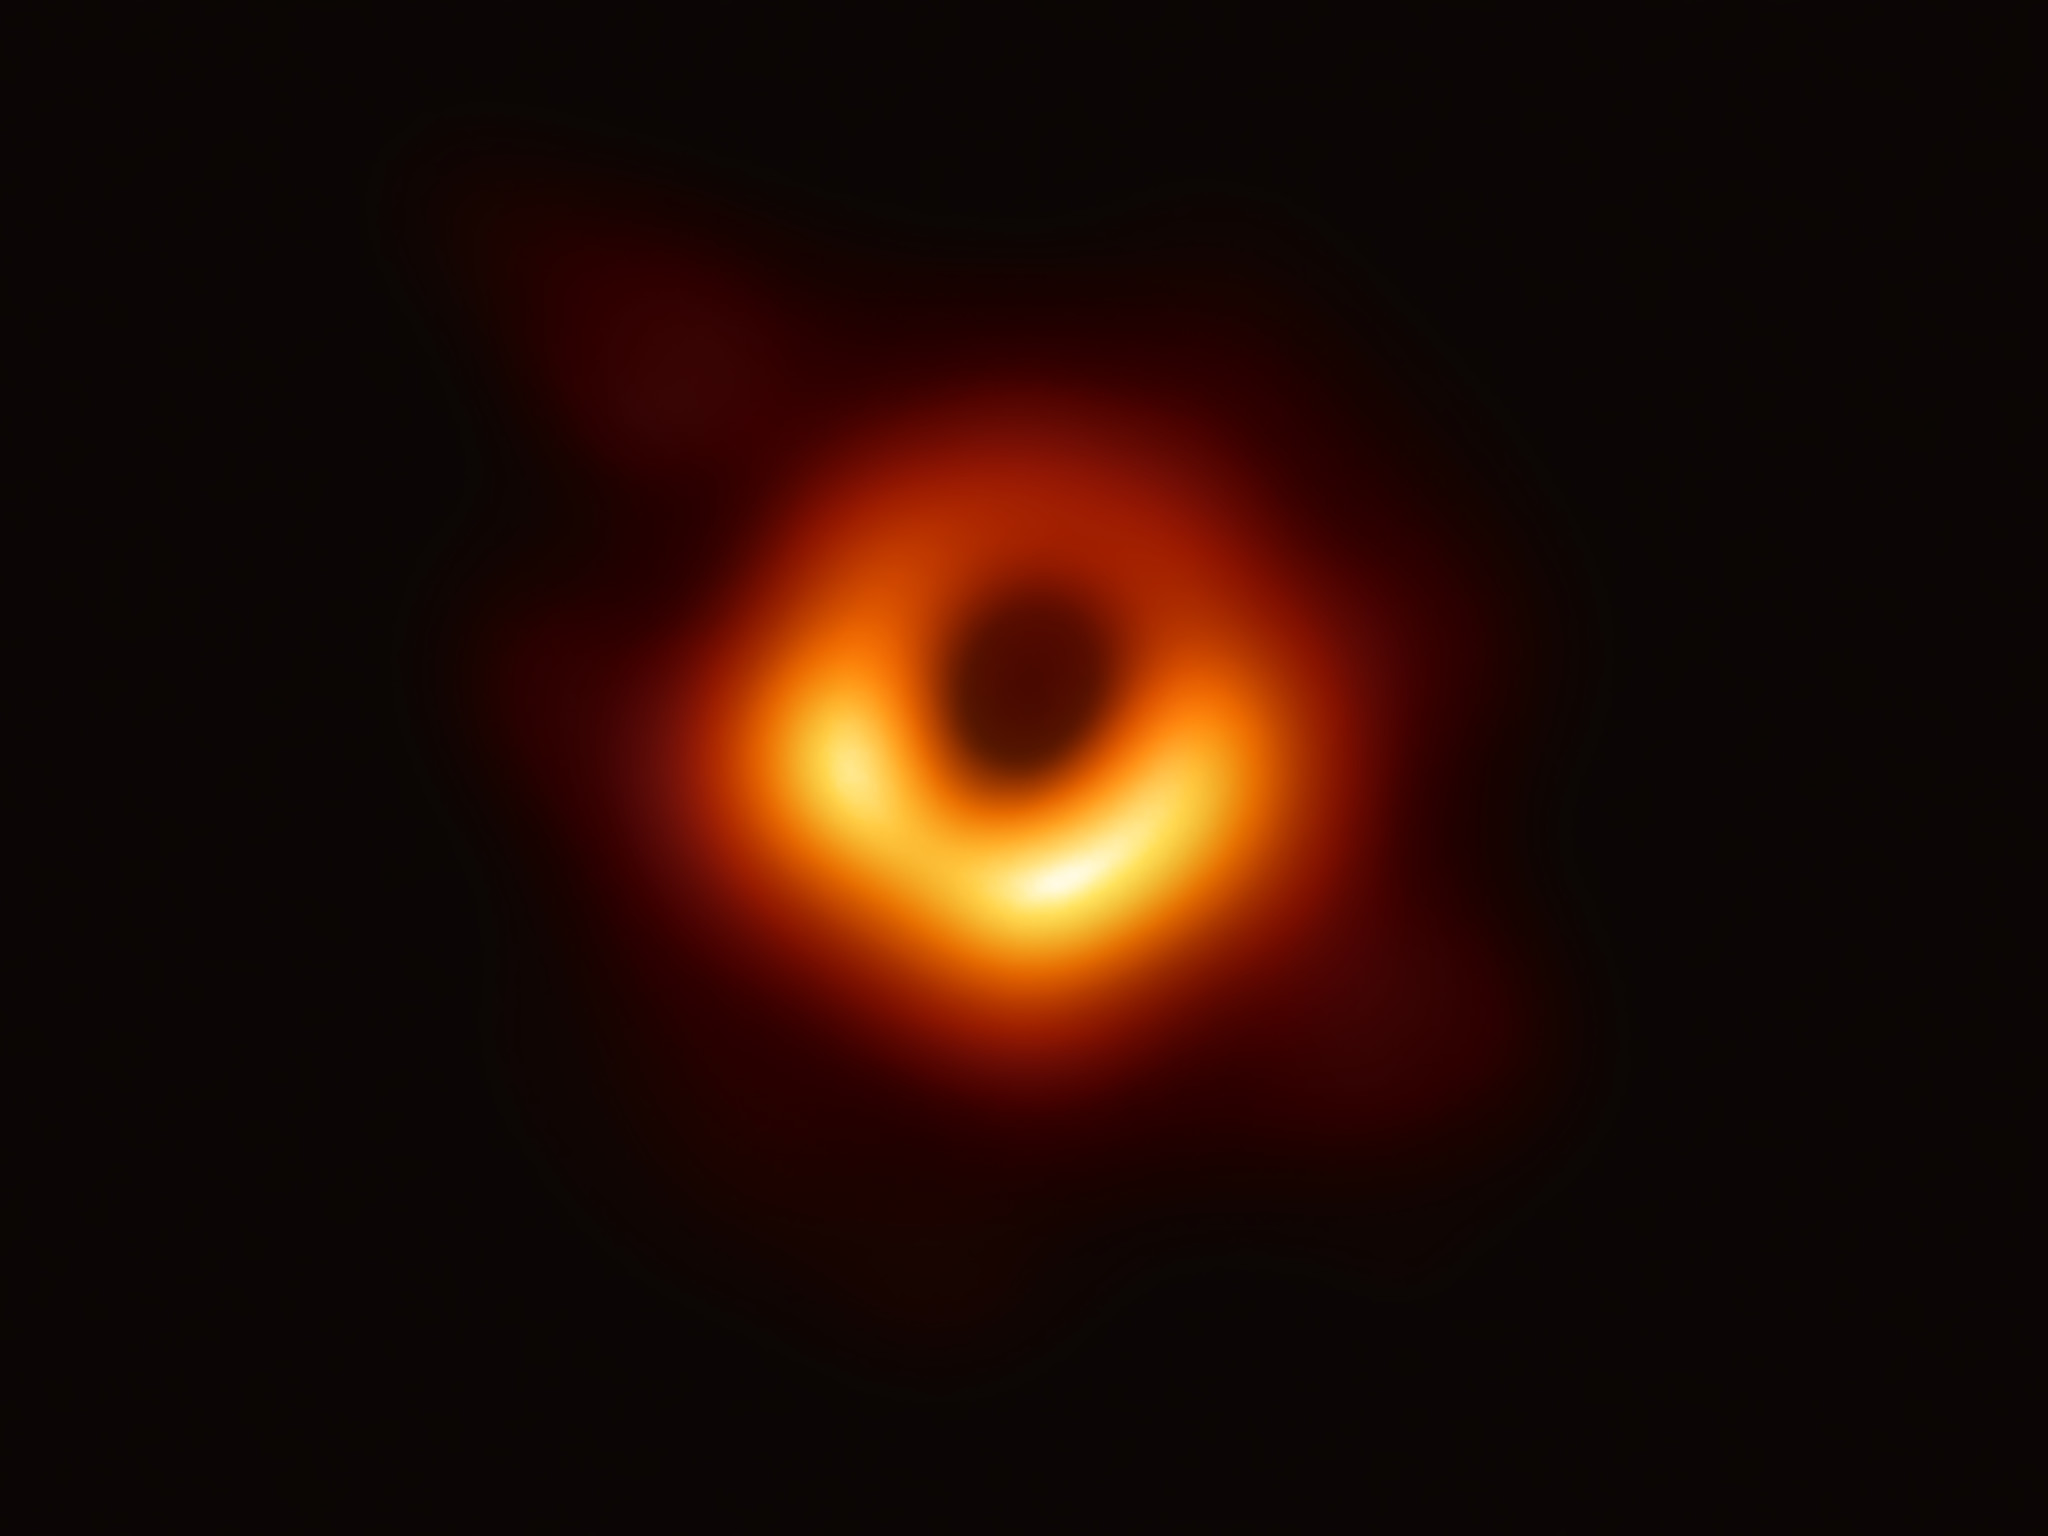
\includegraphics[width=0.4\textwidth]{figures/buconeroimmagine.jpg}
	\caption{Immagine del buco nero raccolta nel 2019}
	\label{fig:figures-buconeroimmagine-jpg}
\end{figure}

Ci sono alcune grandezze in astrofisica che non possono essere dimenticate ai fini di comprendere le grandezze di cui stiamo parlando. Queste grandezze alcune volte vengono anche adottate come unità di misura, visto che nella scala astrofisica le unità standard ridulterebbero decisamente incomprensibili!\\

\subsection{Massa del sole}%
Massa del sole: M\textsubscript{\(\odot\)} = $1.989 \cdot 10^{33}$ g $\approx 2 \cdot 10^{33} g$.\\
La massa minima per una stella è circa 0.08 M\textsubscript{\(\odot\)}\footnote{questa è la massa minima per innescare le reazioni termonucleari, chi non raggiunge queste dimensini (ma si avvicina) è detta Nana Bruna}, la massima si aggira attorno a 100 M\textsubscript{\(\odot\)}. \\
Le galassie hanno circa $10^{11}$ stelle, da cui per ottenere la massa di queste ultime si può mediare la massa a quella del sole con l'adeguato esponente. \\
Abbiamo anche aggregati di stelle (tipo Pleiadi, migliaglia di stelle) e più in là vedremo e studieremo gli ammassi di galassie.

\subsection{Distanze e metodo della parallasse}%
Raggio del sole: $R_{\odot} \approx 7 \cdot 10^{10} cm$.\\
La misura delle distanze in astronomia è complicata. Sono necessarie misure indirette spesso. Se voglio conoscere le dimensioni fisiche di un oggetto (trasformare angolo in distanza) ho bisogno di sapere quanto è distante! 
\paragraph{Metodo della parallasse}%
È l'unica misura diretta di distanza disponibile. È inoltre una misura di tipo geometrico:
\begin{figure}[H]
    \centering
    \incfig{metodo-della-parallasse}
    \caption{\scriptsize Metodo della parallasse: la stella risulta in diversi punti del cielo a seconda della posizione della terra.}
    \label{fig:metodo-della-parallasse}
\end{figure}
\noindent
Negli anni novanta abbiamo mandato un satellite che misurava fino ad un millesimo di secondo d'arco. La missione attuale più importante al riguardo è la GAIA: sta adesso mappando il cielo, quando tra qualche anno avrà finito si arriva a 30 microarcosecondi, purtoppo non si esce ancora dalla galassia con questo metodo.\\
Il metodo consiste in pratica nel vedere lo spostamento angolare dell'oggetto in momenti diversi dell'orbita di rotazione della terra attorno al sole: l'angolo di parallasse $\pi$ è la metà dell'angolo $\theta$
\[
	\frac{\theta}{2} = \pi
.\] 
Se conosciamo il raggio di orbita terrestre possiamo trovare la distanza della stella.\\
Noi conosciamo il raggio dell'orbita terreste medio \footnote{Grazie ad un trasponder radar montato sulla luna}, esso è l'unità astronomica A.U: $R \approx 1.5 \cdot 10^{13}$ cm.
\[
	\tan\left( \pi \right) \approx \pi  = \frac{R}{d}
.\] 

Il sistema solare (fino a nettuno) abbiamo una dimensione di 30 A.U. Fuori dal sistema solare è necessario definire un'altra unità di misura: il Parsec.\\
Un parsec è una distanza tale che la parallasse annua è 1'':
\[
	1 \text{ pc} \approx 3.09 \cdot 10^{18} \text{ cm} \sim 3.2 \text{ anni luce}
.\] 
La stella più vicina a noi ha una parallasse annua di 0.75'' l'anno (Proxima Centauri) che equivale a 1.3 pc. Misurare questi angoli è difficile in generale, gli angoli sono molto piccoli.\\
Le dimensioni di una galassia come la nostra invece sono:\\
\begin{figure}[H]
	\centering
	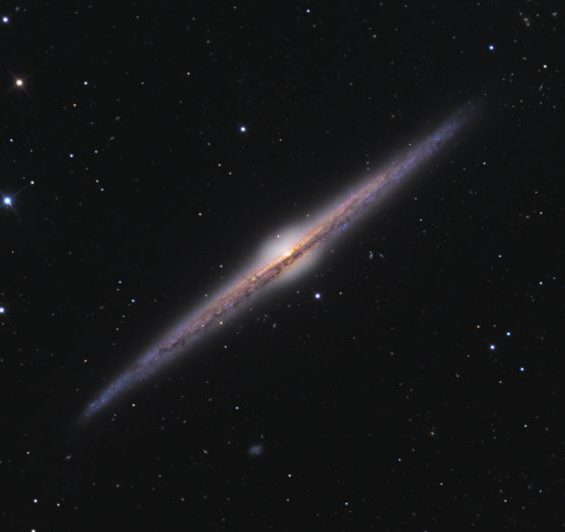
\includegraphics[width=0.4\textwidth]{figures/vialattea.jpeg}
	\caption{Rendering della via lattea vista dall'esterno.}
	\label{fig:figures-vialattea-jpeg}
\end{figure}
\[
	R_{disco} \sim 15 k\text{pc}
.\]
La distanza tra le galassie più vicine tra loro è dell'ordine del Mpc.\\
In genere le stelle invece distano tra loro di quantità dell'ordine dei parsec, è raro che collidano tra loro: l'una tra l'altra sono molto lontane rispetto alle dimensioni delle stelle stesse.\\ 
Non si può dire lo stesso per le galassie, ci sono solo pochi ordini di grandezza tra il raggio galattico è la distanza tra una galassia e l'altra, infatti le collisioni tra galassie sono più frequenti.\\
Le galassie più distanti sono dell'ordine del Gpc (questa è anche la scala delle dimensioni dell'universo).\\
\begin{figure}[H]
    \centering
    \incfig{scale-dell'universo}
    \caption{\scriptsize Scale dell'universo, il disegno è schematico e non è ovviamente in scala.}
    \label{fig:scale-dell'universo}
\end{figure}
\noindent

\subsection{Scale temporali dell'universo}%
Età del sole: $T_{\odot} = 4.57$ Gyr (Giga year). Questa è una delle poche datazioni misurata in modo diretto in astronomia, questa deriva dallo studio delle comete: queste sono rimaste intatte per miliardi di anni, queste vengono datate attraverso radiodatazioni.\\
Età dell'universo (dal Big Bang ad oggi): $T_{uni}= 13.8$ Gyr.

\subsection{Luminosità intrinseca, Candele campioni ed introduzione al trasporto radiativo}%
Negli anni '90 l'ESA ha mandato un satellite in grado di mappare decine di migliaglia di stelle attorno a noi distanti fino a 10 pc. GAIA è l'evoluzione di questo progetto, essa permettera di mappare tridimensionalmente la galassia. \\
Tuttavia anche con GAIA non si esce dalla galassia, quindi come si fa ad uscire? Come si misura la distanza se non sono in grado di misurare la parallasse?\\
Serve un metodo indiretto basato sul'concetto di \texttt{Candela campione}: un oggetto astronomico ci cui conosco la luminosità intrinseca.\\
Confrontando la luminosità intrinseca e la luminosità apparente osservata possiamo dedurre la distanza dell'oggetto. Questo è l'unico modo per misurare le distanze di oggetti all'esterno della via lattea. (Gli oggetti campione sono in genere le supernove).\\
Come faccio a partire dalla luminosità intrinseca a misurare la distanza?
\begin{figure}[H]
    \centering
    \incfig{propagazione-della-radiazione}
    \caption{Propagazione della radiazione}
    \label{fig:propagazione-della-radiazione}
\end{figure}
\noindent
Prendiamo una sorgente che irraggia come in \hyperref[fig:propagazione-della-radiazione]{Figura 8}. 
Se chiamiamo $F\left( r_1 \right) $ il flusso della radiazione che attraversa la superficie sferica concentrica alla sorgente di raggio $r_1$ allora:
\[
	F\left( r_1 \right) 4\pi r_1^2 = F\left( r_2 \right) 4\pi r_2^2 \implies F\left( r_2 \right) = F\left( r_1 \right) \left( \frac{r_1}{r_2} \right) ^2
.\] 
Abbiamo quindi una buona definizione di luminosità se ci mettiamo sul raggio $R$ della stella che irraggia:
\[
	F\left( R \right) 4\pi R^2  = L
.\] 
Tuttavia questa a livello pratico non è sufficiente. La radiazione non si propaga nel vuoto, è indispensabile quindi costruire una teoria del trasporto radiativo per tener di conto del mezzo interstellare. \\
Dobbiamo introdurre alcune grandezze per studiare il trasporto radiativo: \texttt{Intensità specifica monocromatica} (trattata dal punto di vista macroscopico \footnote{Valido quando la lunghezza d'onda che stiamo studiando sono piccole rispetto alle dimensioni del sistema, questo ci permette di immaginare che la radiazione si propaghi lungo dei raggi}):
\begin{figure}[H]
    \centering
    \incfig{figura-per-introdurre-lintensit-specifica}
    \caption{Figura per introdurre l'intensità specifica}
    \label{fig:figura-per-introdurre-lintensit-specifica}
\end{figure}
\noindent
Supponiamo di essere in un punto $\bs{r}$ all'istante $t$ e prendiamo in questo punto una superficie infinitesima elementare $dA$ orientata nella direzione $\hat{n}$ come in \hyperref[fig:figura-per-introdurre-lintensit-specifica]{Figura 9}. Ci interessa calcolare l'energia trasportata dalla radiazione elettromagnetica che attraversa la superficie $dA$ nella direzione $\hat{k}$ all'interno dell'angolo solido $d\Omega$ (inoltre deve essere monocromatica: tra $\nu$ e $d\nu$).\\
Quello che cerchiamo è dato da:
\[
	dE = I_{\nu}\left( \bs{r}, t,\bs{k} \right) \hat{k}\hat{n} dAdtd\Omega d\nu
	= I_{\nu}\left( \bs{r},t, \bs{k} \right) \cos\theta dA dt d\Omega d\nu
.\] 
Questa quantità è un flusso per unità di angolo solito: una brillanza superficiale. 
\[
	[I_{v}] = \text{[erg] cm $^{-2}$ s $^{-1}$ ster $^{-1}$ Hz $^{-1}$} 
.\] 
Dove ster è lo ster radiante.\\
$I_{\nu}$ è l'energia trasportata da un gruppo di fotoni che si muovono tutti nella stessa direzione contemporaneamente e tutti con la stessa frequenza.\\
È necessario notare che l'interazione tra radiazione e materia è anche argomento microscopico: il fotone interagisce anche con ioni, protoni, nuclei nel suo tragitto. Terremo conto con opportuni coefficienti il passaggio della radiazione nei vari mezzi quando scriveremo l'equazione del trasporto.\\

\lez{2}{24-02-2020}{}
Riprendiamo la teoria del trasporto radiativo.
\[
	dE = I_{\nu}\left( \bs{r}, t,\bs{k} \right) \hat{k}\hat{n} dAdtd\Omega d\nu
.\] 
Conoscere il campo di radiazione in una determinata regione significa conoscere l'intensità specifica del campo di radiazione: $I_{\nu}\left( \bs{r}, t,\bs{k} \right)$.\\ 
Tale quantità ricordiamo essere un flusso per unità di angolo solido. Presa una superficie infinitesima dA come nella lezione precedente:
\begin{figure}[H]
    \centering
    \incfig{figura-per-introdurre-lintensit-specifica}
    \caption{Figura per introdurre l'intensità specifica}
    \label{fig:figura-per-introdurre-lintensit-specifica}
\end{figure}
\noindent
L'energia trasportata dalla radiazione elettromagnetica tra la frequenza $\nu$ e $\nu + d\nu$ che attraversa la superficie $dA$ è data dalla relazione con cui abbiamo introdotto questa lezione.\\
Questa $I_{\nu}\left( \bs{r}, t, \bs{k} \right)$ non descrive completamente il campo di radiazione: lo descrive nei confini dell'ottica geometrica. No tiene di conto infatti di fenomeni come interferenza e diffrazione. Anticipiamo che nella maggior parte delle situazioni di interesse la quantità $I_{\nu}\left( \bs{r}, t,\bs{k} \right)$ non dipende dal tempo perchè il campo di radiazione ed il mezzo stesso sono in genere stazionari \footnote{Ci sono anche casi in cui questo non è vero, nei casi che affrontiamo noi invece lo daremo per scontato.}. \\
\subsection{Momenti dell'intensità $I_{\nu}$}%
Spesso inoltre non serve conoscere direttamente  $I_{\nu}\left( \bs{r}, t,\bs{k} \right)$, bastano altre quantità con meno informazioni. Facciamo in questa sezione alcuni esempi.
\paragraph{Flusso}%
Immaginiamo di volere il flusso  $F_{\mu}$ monocromatico (tra la frequenza $\nu$ e $\nu + d\nu$) attraverso la superficie $dA$ nell'unità di tempo, calcoliamo dapprima la radiazione che si propaga nella direzione $\bs{k}$ che chiamiamo $\phi$:
\begin{align}
	\phi = \frac{\mbox{d} E}{\mbox{d} A \text{d}t} = \frac{I_{\nu}\cos\theta}{dA dt} dA dt d\Omega d\nu = I_{\nu} \cos\theta d\Omega d\nu
.\end{align}
Per ottenere il flusso basterà integrare in tutto l'angolo solido ottenendo:
\[
	F_{\nu} = \int_{\Omega} I_{\nu}\cos\theta d\Omega \ \left[ \text{erg} \right]  \left[ \text{cm} \right]^{-2} \left[ s \right]^{-1} \left[ \text{Hz} \right]^{-1} 
.\] 
Se vogliamo il flusso totale sarà necessario integrare nelle frequenze:
\[
	F = \int F_{\nu} d\nu
.\] 
Chiaramente nel flusso cè meno informazione che nella intensità specifica perchè abbiamo perso informazioni sull'angolo e quindi sulla direzione di propagazione.\\
Notiamo che nei casi in cui la radiazione è isotropa il flusso sarà nullo: la quantità di radiazione che va verso l'alto è la stessa di quella verso il basso \footnote{Infatti l'integrale fa proprio zero, poichè tutto esce dall'integrale in $\Omega$ tranne il coseno, mentre l'elemento infinitesimo di angolo solido è proporzionale a $\sin\theta d\theta$}.\\
Un esempio di radiazione isotropa è quella di corpo nero. Per tale oggetto, inserendo in rilevatore all'interno della famosa cavità rileviamo appunto un flusso nulla.\\
In natura una ottima approssimazione di corpo nero sarà l'interno delle stelle.\\
\paragraph{Densità di energia irraggiata}%
Un'altra quantità che si può ricavare quando è noto $I_{\nu}$ è la densità di energia $u_{\nu}$:
consideriamo l'elementino di volume composto dalla quantità di radiazione che attraversa l'area $dA$ nel tempo $dt$ facendo sempre riferimento alla \hyperref[fig:figura-per-introdurre-lintensit-specifica]{Figura 10}:
\[
	dV = dA \cos\theta c dt 
.\] 
si ha che, ragionevolmente, la densità di energia sarà parente della quantità:
\[
	\frac{\mbox{d} E}{\mbox{d} V} = \frac{I_{\nu}\left( \bs{r}, t, \bs{k} \right)  \hat{k} \cdot \hat{n} dA dt d\Omega d\nu}{dA \cos\theta c dt} = \frac{I_{\nu}}{c}d\Omega d\nu
.\] 
Dove abbiamo usato il fatto che $\hat{k}\cdot \hat{n} =\cos\theta$.\\
Basta adesso integrare sull'angolo solido per ottenere $u_{\nu}$:
\[
	u_{\nu} = \int \frac{I_{\nu}}{c}d\Omega \quad \left[ \text{erg} \right] \left[ \text{cm} \right]^{-3} \left[ \text{Hz} \right]
.\] 
Se la radiazione è isotropa $I_{\nu} /c$ può uscire dall'integrale:
\[
	u_{\nu} = \frac{I_{\nu}}{c} \int d\Omega = \frac{4\pi}{c} I_{\nu} 
.\]
Nel caso del corpo nero abbiamo, dalla legge di radiazione di Plank che:
\[
	u_{\nu} = \frac{8\pi\hbar}{c^3} \frac{\nu^3}{e^{\frac{\hbar \nu}{kT}}-1}= \frac{4\pi}{c} B_{\nu}
.\] 
Dove abbiamo introdotto la quantità:
\[
	B_{\nu}= \frac{2 \hbar}{c^2} \frac{\nu^3}{e^{\frac{\hbar \nu}{kT}}-1}
.\] 
\paragraph{Pressione}%
Possiamo trovare la pressione della radiazione calcolando il flusso della componente ortogonale della quantità di moto alla superficie attraversata $dA$:
\[
	\bs{p}_{\bot} \cdot \hat{n}=\frac{dE}{c}\hat{k}\cdot \hat{n}= \frac{I_{\nu} \cos^2\theta}{c} \frac{dA dt}{dA dt} d\Omega d\nu = \frac{I_{\nu}}{c}\cos^2\theta d\Omega d\nu
.\] 
Dove abbiamo sfruttato che i fotoni sono particelle senza massa per relazionare l'energia alla quantità di moto.
Quindi abbiamo che, integrando nell'angolo solido come sopra si ottiene la pressione per unità di frequenza: 
\[
	P_{\nu} = \int \frac{I_{\nu}}{c} \cos^2\theta d\Omega 
.\] 
E integrando ancora nella prequenza si ottiene la pressione:
\[
	P = \int P_{\nu}d\nu 
.\] 
Notiam adesso che se il campo è isotropo il risultato che otteniamo è il seguente:
\[
	 P = \frac{4\pi}{3}\frac{I_{\nu}}{c} = \frac{u_{\nu}}{3}
.\] 
Nel caso degli interni stellari \footnote{che sono la cosa che approssima meglio il corpo nero dopo l'universo stesso.} avviciniandoci verso il centro delle stelle non si ha esattamente un irraggiamento isotropo per il semplice motivo che questo richiederebbe un equilibrio termodinamico esatto. Ci sarà invece un gradiente di temperatura andando verso il centro della stella, quindi ci aspettiamo anche in questa situazione una anisotropia nella radiazione.\\
Tale anisotropia sarà così piccola che per la maggior parte delle applicazioni che vedremo può essere trascurata, tuttavia globalmente non può essere trascurata perchè proprio quella lieve luce che noi vediamo guardando il cielo notturno.

\paragraph{Intensità specifica media sull'angolo.}%
\[
	J_{\nu} = \frac{\int I_{\nu}d\Omega}{4\pi}
.\] 
Nel caso del campo isotropo si ha: $J_{\nu} = I_{\nu}$.\\
È possibile esprimere la densità di energia in termini di $J_{\nu}$ :
\[
	u_{\nu} = \frac{4\pi}{c}J_{\nu}
.\] 
\paragraph{Momenti dell'intensità}%
Tutti gli oggetti ricavati sono stati estrapolati con la forma:
\[
	\int I_{\nu} \cos^{n}\theta d\Omega
.\] 
Questi sono detti i momenti di ordine (0,1,2) dell'intensità specifica $I_{\nu}$, riguardando quanto fatto sopra possiamo notare che i tre esempi che abbiamo fatto sono:
\begin{itemize}
	\item $u_{\nu}$ : momento di ordine 0 di $I_{\nu}$.
	\item $F_{\nu}$ : momento di ordine 1 di $I_{\nu}$.
	\item $P_{\nu}$ : momento di ordine 2 di $I_{\nu}$.
\end{itemize}
Quindi data la forma funzionale della intensità specifica \footnote{vedremo che basta l'equazione per quest'ultima, che si chiamerà equazione del trasporto.} possiamo possiamo ricavare tutti i momenti della quantità stessa. L'utilità di questi momenti è che possono isolare e rendere applicabili informazioni utili sul sistema.\\

\subsection{Propagazione di un fascio nel vuoto.}%
Vogliamo vedere che cosa succede all'intensità specifica di un fascio che si propaga nel vuoto.\\
Abbiamo visto che il flusso di un fascio che si propaga nel vuoto scala come $R^{-2}$, quindi il flusso della sorgente è sempre più debole mano a mano che la sorgente si allontana.\\ 
Per l'intensità specifica invece si ha che visivamente resta costante: mentre l'auto si allontana ci sembra che il suo brillare non cambi. Vediamo se si può dimostrare questo fatto, consideriamo il seguente caso:
\begin{figure}[H]
    \centering
    \incfig{brillanza-costante}
    \caption{\scriptsize Sistema in cui osservo la radiazione da una sorgente.}
    \label{fig:brillanza-costante}
\end{figure}
\noindent
Il fascio si propaga nella direzione $\bs{k}$ e noi vogliamo sapere come cambia $I_{\nu}$ lungo questa direzione, per questo prendiamo due punti lungo $\bs{k}$ che in figura chiamiamo $\bs{r}$ e $\bs{r}'$ e valutiamo la brillanza in tali pundi: cerchiamo la quantità di radiazione che attraversa le aree infinitesime associate ai due punti $dA$ e $dA'$.
Ipotizziamo infatti che la sorgente si nella parte destra della figura, allora la luce proveniente da $dA$ che arriva alla posizione $\bs{r}'$ è quella sottesa all'angolo solido $d\Omega'$, d'altra parte la luce che arriva a $\bs{r}$ e che passa poi dall'area $dA'$ è senza dubbio quella sottesa all'angolo solido $d\Omega$.
Per farlo sfruttiamo gli angoli solidi costruiti in Figura \ref{fig:brillanza-costante}. Gli angoli solidi costruiti in figura possono essere scritti come:
\[
	d\Omega = dA' \frac{\hat{n}'\cdot \hat{k}}{s^2}
.\] 
\[
	d\Omega' = dA \frac{\hat{n}\cdot \hat{k}}{s^2}
.\] 
E l'energia trasportata dalla radiazione elettromagnetica nei due casi è, per definizione:
\begin{align}
	&dE' = I_{\nu}\left( \hat{k}', t', \bs{r}' \right) \hat{k}'\cdot \hat{n}' dt d\Omega d\nu dA'\\
	&dE = I_{\nu}\left( \hat{k}, t, \bs{r}\right) \hat{k}\cdot \hat{n} dt d\Omega' d\nu dA
.\end{align}
Se la radiazione si propaga nel vuoto allora l'energia si deve conservare, quindi $dE = dE'$. Quindi inserendo anche gli angoli solidi ricavati sopra si ottiene un risultato importante:
\[
	I_{\nu}\left( \bs{r}, t, \hat{k} \right) =I_{\nu}\left( \bs{r}', t, \hat{k}' \right)
.\] 
La conservazione della brillanza. Possiamo allora scrivere la legge di conservazione per questa quantità nel vuoto:
\[
	\frac{1}{c}\frac{\partial I_{\nu}}{\partial t} + \frac{\partial I_{\nu}}{\partial s}  = 0
.\] 
in cordinate cartesiane la legge si scrive:
\[
	\frac{\partial I_{\nu}}{\partial s} =
	\frac{\partial x}{\partial s} \frac{\partial I_{\nu}}{\partial x} + 
	\frac{\partial y}{\partial s} \frac{\partial I_{\nu}}{\partial y} +
	\frac{\partial z}{\partial s} \frac{\partial I_{\nu}}{\partial z}= 
	k_{x} \frac{\partial I_{\nu}}{\partial x} + 
	k_{y}\frac{\partial I_{\nu}}{\partial y} + 
	k_{z}\frac{\partial I_{\nu}}{\partial z}  
.\] 
Questo entra in conflitto con il fatto che il flusso scala come $R^{-2}$? No, perchè l'intensità specifica è un flusso per unità di angolo solido. \\
Prendiamo una sorgente luminosa che siamo in grado di risolvere (vedo la forma geometrica), ipotizzaimo che la sorgente si allontana da noi, la sorgente risulterà sempre più piccola \footnote{Ipotizziamo che non ci sia nebbia, in modo da avvicinarci il più possibile ad una situazione di vuoto}.\\
Tuttavia, finche riusciamo a risolverlo il faro risulterà brillante allo stesso modo. Questo perchè è vero che il flusso diminuisce come $R^{-2}$ ma è anche vero che  l'angolo solido si riduce della stessa quantità $R^{-2}$, quindi resta invariatà la quantità $I_{\nu}$. Possiamo quindi affermare che la brillanza si conserva lungo il raggio.\\
Se vogliamo, questa è la controparte macroscopica di un fatto microscopico: se un fotone viaggia nel vuoto la probabilità che decada è nulla.\\
Esempio astronomico: una sorgente che possiamo risolvere sono le galassie. Tuttavia non riusciamo a risolvere per le stelle perchè per noi sono oggetti puntiformi.\\
Quindi quando vediamo una luce proveniente da una stella noi vediamo la sua diffrazione, non la vera forma. Quindi l'estensione andolare dipende dalla legge di diffrazione.\\
Quindi non possiamo applicare il ragionamento che abbiamo fatto in precedenza se non siamo in grado di risolvere la sorgente.\\
\paragraph{Esempio classico}%
Supponiamo di avere una sorgente sferica uniformemente brillante: ogni raggio uscente ha la stessa intensità specifica $I$:
 \[
	I = \begin{cases}
		&B  \ \text{ Se il raggio interseca la superficie}\\
		&0 \ \text{ Altrimenti}
	\end{cases}
.\] 
\begin{figure}[H]
    \centering
    \incfig{esempio-su-conservazione-della-brillanza}
    \caption{Esempio sulla conservazione della brillanza}
    \label{fig:esempio-su-conservazione-della-brillanza}
\end{figure}
\noindent
Calcoliamo il flusso al punto P \footnote{Ovvero il flusso sotteso all'angolo solido costruito a partire da $P$ verso la sorgente}:
\begin{align}
	F =& \int I\cos\theta d\Omega=\\
	  =&\int_{0}^{2\pi}d\varphi \int_{0}^{\theta_{c}}B \cos\theta\sin\theta d\theta =\\
	  =&2\pi B\frac{1-\cos^2\theta_{c}}{2}=\\
	  =&\pi B \sin^2\theta_{c}=\\
	  =&\pi B \left( \frac{R}{r} \right) ^2
.\end{align}
Se abbiamo una sorgente uniformemente brillante e isotropa il flusso che esce alla superficie è dato da:
\[
	F = \pi B
.\] 
Non è zero perchè questo è il flusso uscente, non sull'angolo solido come invece abbiamo visto prima.\\
\subsection{Propagazione della radiazione in un mezzo}%
Vogliamo vedere come cambia interagendo con la materia $I_{\nu}$, sicuramente non rimarrà costante perchè la radiazione interagisce con la materia: una parte dei fotoni verranno sottratti al fascio ed altri fotoni verranno immessi nel fascio. \\
Il nostro obbiettivo è quantificare il bilancio tra i primi fenomeni detti Pozzi ed i secondi dette Sorgenti.\\
\texttt{L'equazione del trasporto} sarà della forma:
\[
	\frac{1}{c}\frac{\partial I_{\nu}}{\partial t} + \hat{k} \nabla I_{\nu} = + \left\{ \text{processi di sorgenti} \right\} - \left\{ \text{Processi di pozzi} \right\} 
.\] 
È quindi indispendabile conoscere i meccanismi di interazione tra la radiazione e la materia, la distanza percorsa dal fascio all'interno del mezzo e le condizioni del mezzo stesso.\\
Non dobbiamo sottovalutare il fatto che i fotoni stessi modificano lo stato del mezzo, quindi i fotoni ed il mezzo possono influenzarsi a vicenda. Per questo l'equazione del trasporto diventa con grande facilità non lineare. \\
Prendiamo quindi il seguente schema come riferimento:
\begin{figure}[H]
    \centering
    \incfig{radiazione-in-un-mezzo}
    \caption{Radiazione in un mezzo}
    \label{fig:radiazione-in-un-mezzo}
\end{figure}
\noindent
Al momento dell'ingresso (alla coordinata $s_0$) la brillanza vale: $I_{\nu}\left( s_0 \right)$  e sarà uguale a quella della sorgente in tal punto.
\paragraph{Esempi di processi di emissione o di assotbimento}%
Potremmo considerare lo scattering tra questi meccanismi, anche se vedremo che questi sono fastidiosi: aggiungono un elemento di non località alla nostra indagine sulla radiazione.\\ 
Quest'ultima affermazione può essere giustificata con un esempio: supponiamo di voler visualizzare lo spettro che proviene dalla faccia di una persona all'aperto sotto la luce del sole \footnote{Di fatto significa prendere la luce riflessa sulla faccia della persona}. \\
Dall'analisi troverei il doppietto del sodio. Tuttavia è difficile che le condizioni fisiche sulla faccia di una persona sono tali da vedere il doppietto del sodio. Ci si chiede allora come sia possibile vederlo nel volto della persona. La risposta sta nel fatto che la luce che viene dalla faccia è nata sulla superficie del sole, le righe del doppietto del sodio arrivano proprio dalla atmosfera del sole.\\
Quindi le righe che visualizziamo sono state create in situazioni completamente diverse rispetto alle condizioni fisiche del sistema dalla quale preleviamo la luce (il volto). Questo quindi perchè le proprietà del fotone scatterato contiene informazioni che nella maggior parte dei casi non ci sono utili a studiare il sistema locale che in questo caso è un volto.\\
Un'altro effetto che produce fotoni è l'emissione da eccitazione, tra poco distingueremo tra i tipi di emissione \footnote{Che a seconda della situazione possono comportarsi da pozzi o da sorgenti}. \\
Un processo di assorbimento è invece la  fotoionizzazione: il passaggio da un livello energetico ad un livello del continuo.\\
\paragraph{Distinzione tra processi di emissione e di assorbimento}%
Se abbiamo un fotone che incide su un atomo e sparisce senza dare luogo ad un fotone la cui direzione è correlata a quella del fotone incidente allora si dice che è avvenuto un fenomeno di assorbimento.\\
Se il fotone sparito eccita un atomo può succedere che questo, ad un certo punto, si disecciti. Se l'atomo quando perde l'eccitazione ha perso memoria di quanto gli era successo in precedenza allora avviene una emissione scorrelata, se invece l'atomo si diseccita prima di perdere memoria della eccitazione \footnote{Quindi prima di urtare altri atomi, ad esempio.} allora si parla di emissione correlata.\\
Nei casi di nostro interesse gli urti saranno talmente tanti che possiamo considerare i fotoni generati tutti scorrelati.\\
Potremmo anche distinguere tra assorbimenti in scattering ed assorbimenti termici, dove i primi gli abbiamo discussi sopra, i secondi invece sono quelli in cui i fotoni vanno ad eccitare il materiale aumentandone la temperatura. Nel caso di assorbimenti termici il nostro raggio va a trasferire energia al mezzo, cambiandone le condizioni fisiche.\\
\subsection{Equazione del trasporto: processi di interazione radiazione materia}%
\paragraph{Emissione}%
Consideriamo adesso i processi di emissione e prendiamo un elementino di volume $dV$ contenuto nel mezzo: 
\begin{figure}[H]
    \centering
    \incfig{elemento-di-volume-del-mezzo}
    \caption{Elemento di volume del mezzo}
    \label{fig:elemento-di-volume-del-mezzo}
\end{figure}
\noindent
Secondo la notazione in figura si ha che: $dV = ds\cdot dA$.\\
Definiamo il coefficiente di emissione monocromatico $j _{\nu}$ tale che la quantità di energia che viene messa dal mezzo di volume $dV$ nell'intervallo di tempo dt e nell'angolo solido $d\Omega$ è data da:
\[
	dE = j _{\nu} dV dt d\Omega d\nu
.\] 
Questi sono coefficienti macroscopici, per calcolarli dovremmo fare il conto di tutti i processi microscopici ed inserirli nel conto. Quindi dal punto di vista della fisica è un termine pesantissimo da trovare.\\
Le unità di questo oggetto sono: $\left[ j _{\nu} \right] = \left[ \text{erg} \right] \cdot \left[ \text{cm} \right]^3 \cdot \left[ \text{s} \right]^{-1} \cdot \left[ \text{sterad} \right]^{-1} \cdot \left[ \text{Hz}^{-1} \right]$.
Vediamo come viene modificato il mezzo dall'emissione dovuta a questo termine, ovvero dall'emissione del mezzo. Facciamo riferimento alla Figura \ref{fig:elemento-di-volume-del-mezzo}.\\
Possiamo scrivere la quantità di energia che esce dal volumetto $dV$ :
\[
	dE_{\text{out}} = I_{\nu}\left( s+ds, t+dt, \hat{k} \right) dA dt d\Omega d\nu
.\] 
mentre nel punto di ingresso avremo
\[
	dE_{\text{in}} = I_{\nu}\left( s, t, \hat{k} \right) dA dt d\Omega d\nu
.\] 
La differenza tra le due sarà l'energia prodotta nei processi di emissione per la conservazione di energia.
\begin{align}
	dE_{\text{out}}- dE_{\text{in}} =& \left( I_{\nu}\left(s+ds,t+dt,\hat{k}\right)-I_{\nu}\left(s,t,\hat{k}\right)\right)dt\cdot dA\cdot d\Omega\cdot  d\nu = \\
	=& \left[ \frac{1}{c}\frac{\partial I_{\nu}}{\partial t} + \frac{\partial I_{\nu}}{\partial s}  \right] ds\cdot dA\cdot dt\cdot d\Omega\cdot  d\nu  \\
.\end{align}
In cui abbiamo sostituito la variazione quadridimensionale di $I_{\nu}$ nell'ultimo passaggio, adesso ricordando che questa differenza di energia deve essete uguale alla energia emessa possiamo imporre l'uguaglianza:
\[
	\left[ \frac{1}{c}\frac{\partial I_{\nu}}{\partial t} + \frac{\partial I_{\nu}}{\partial s}  \right] ds\cdot dA\cdot dt\cdot d\Omega\cdot  d\nu  = 
	j _{\nu} dA \cdot ds\cdot  dt\cdot  d\Omega\cdot  d\nu
.\] 
Quindi se il mezzo è stazionario allora si ha che $\frac{\partial I_{\nu}}{\partial t} = 0$, quindi abbiamo che:
\[
	j _{\nu}= \frac{\partial I_{\nu}}{\partial s} 
.\] 
Il termine trovato ci dice come cambia l'intensità specifica nel mezzo. Quindi se c'è soltanto emissione ci aspettiamo che l'intensità specifica aumenti perchè in tal caso $j_{\nu}$ è positivo.
\paragraph{Assorbimento}%
Possiamo definire l'assorbimento in modo analogo al caso precedente, per quest'ultimo però è necessario inserire l'intensità specifica in ingresso.\\
Infatti l'emissione può esistere in presenza o in assenza del campo di radiazione, l'assorbimento no.\\
Il coefficiente di assorbimento vero $\alpha_{\nu}$ è definito a partire dalla quantità di energia sottratta per assorbimento:
\[
	dE = \alpha_{\nu} I_{\nu} dA \cdot ds\cdot dt\cdot d\Omega\cdot d\nu
.\] 
Questo coefficiente ha le dimensioni $\left[ m \right]^{-1}$, l'inverso di questa quantità è il cammino libero medio monocromatico nel mezzo per la radiazione.
\\Quindi facendo i conti come in precedenza di arriva a:
\[
	\left[ \frac{1}{c}\frac{\partial I_{\nu}}{\partial t} + \frac{\partial I_{\nu}}{\partial s}  \right] = -\alpha_{\nu} I_{\nu}
.\] 
Il segno è dovuto al fatto che adesso l'energia che entra è maggiore dell'energia che esce, quindi abbiamo inserito un segno negativo.\\
Quindi la convenzione è che $\alpha_{\nu}$ è positivo \footnote{Siccome esistono anche i processi di emissione stimolata essi verranno considerati nel termine di assorbimento come correzioni di ordine maggiore di segno negativo, per questo puntualizziamo la convenzione sul segno.}. Quindi se c'è solo assorbimento vero il raggio si affievolisce nel passaggio attraverso il mezzo, come ci si potrebbe aspettare.
\paragraph{Scattering}%
Per quanto riguarda i pozzi si ha lo scattering per cui i fotoni uscenti sono incoerenti con la radiazione entrante, come spiegato sopra. Per questo fenomeno si introfuce un coefficiente $-\alpha_{\nu}^{\text{scatt}}$ moltiplicato per $I_{\nu}$.\\
Per i pozzi invece abbiamo da considerare il fatto che il fotone uscente dallo scattering potrebbe essere emesso in tutte le direzioni, sarà necessario introdurre l'integrale di tutti i fotoni che si stanno muovendo lungo una qualunque direzione ($\hat{k}'$) e che vengono scatterati nella direzione del fascio $\hat{k}$ integrando su tutto l'angolo solido:
 \[
	 \alpha_{\nu}^{\text{scatt}}\int\phi\left( \hat{k},\hat{k}' \right) I_{\nu}\left( \hat{k}' \right) d\Omega
.\] 
Dove $\phi\left( \hat{k}.\hat{k}' \right)$ è la densità di probabilità che un fotone venga emesso nella direzione $\hat{k}$.
\paragraph{Equazione finale con tutti i termini}%
\[
	\left[ \frac{1}{c}\frac{\partial I_{\nu}}{\partial t} + \frac{\partial I_{\nu}}{\partial s}  \right] =
	j _{\nu} 
	- \alpha_{\nu}I_{\nu} 
	- \alpha_{\nu}^{\text{scatt}}I_{\nu} 
	+ \alpha_{\nu}^{\text{scatt}} \int\phi\left( \hat{k},\hat{k}' \right) I_{\nu}\left( \hat{k}' \right) d\Omega
.\] 
Abbiamo quindi una equazione integro differenziale molto complicata da risolvere. L'incognita da calcolare è l'intensità specifica.\\
In realtà la faccenda è ancora più  complessa: i coefficienti di solito nemmeno si conoscono! Per tutte le specie atomiche e per tutti i livelli di ciascuna bisognerebbe calcolare le probabilità dei singoli processi.


\lez{3}{27-02-2020}{}
Per completare il quadro dei coefficienti dobbiamo aggiungere, nel caso dell'emissione isotropa si usa il coefficiente di emissività $\epsilon _{\nu}$. Il coefficiente di emissività è l'analogo del coefficiente di emissione per unità di massa. \\
Nel caso di radiazione isotropa il legame tra questo coefficiente ed il coefficiente di emissione può essere espresso mediante la seguente:
\[
	j _{\nu} = \frac{\epsilon _{\nu} \rho }{4\pi}
.\] 
Quindi in tal caso possiamo esprimere la variazione di energia come:
\[
	dE = j _{\nu}dVdtd\Omega d\nu= \epsilon_{\nu}\rho dV dt \frac{d\Omega}{4\pi}dV
.\] 
Inoltre abbiamo la sezione d'urto $\sigma _{\nu} $ delle particelle che assorbono fotoni, possiamo dimostrare che questa è legato a $\alpha _{\nu} $. Prendiamo il volumetto di materiale attraversato:
\begin{figure}[H]
    %This is a custom LaTeX template!
    \centering
    \incfig{dimostrazione-sigma-nu}
    \caption{\scriptsize Elemento infinitesimo di materiale attraversato.}
    \label{fig:dimostrazione-sigma-nu}
\end{figure}
\noindent
Abbiamo gia definito la quantità di energia sottratta al fascio dal materiale:
\[
	dE = \alpha _{\nu} I_{\nu} dV dt d\Omega d\nu 
.\] 
Immaginiamo che il nostro mezzo sia costituito da particelle tutte uguali e tutte in grado di assorbire la radiazione, supponiamo che la sezione d'urto di assorbimento di ogni particella sia $\sigma _{\nu} $. Le particelle per unità di volume saranno: $dN = n dV = n dA ds$. Nelle ipotesi in cui il gas sia sufficientemente rarefatto:
\[
	\sqrt{\sigma _{\nu}} \ll d
.\] 
Con d distanza tra le particelle. Possiamo immaginare che le particelle del gas non si occultino l'una con l'altra, quindi la superficie assorbente complessiva sarà la somma di tutte le sezioni d'urto di ogni singola particella. Essendo le particelle tutte uguali otteniamo che $dA' = \sigma _{\nu} dN = \sigma _{\nu} dA ds$.\\
Abbiamo detto che un fotone viene assorbito su $\sigma _{\nu} $, allora nel volumetto i fotoni che vengono assorbiti sono solo quelli che incidono sulla superficie $dA'$. L'energia che viene sottratta al fascio dal materiale sarà quella che incide su questa superficie $dA'$ e visto che l'energia che attraversa tale superficie può sempre essere espressa tramite:
\[
	dE_{sott} = I_{\nu} dA' dt d\Omega d\nu 
.\] 
Possiamo eguagliare questa all'energia persa per assorbimento:
\[
	dE = \alpha _{\nu} dN dt d\Omega d\nu 
.\] 
ottenendo la legge:
\[
	\alpha_{\nu} = n \sigma_{\nu}
.\] 
Un'altra quantità utilizzata è l'opacità radiativa $k_{\nu}$, questa è legata ad $\alpha_{n}$ tramite: $\alpha_{\nu}= k_{\nu}\cdot \rho$. Questa quantità è una sezione d'urto per unità di massa, calcolarla è molto difficile.\\
Torniamo adesso alla quantità $j _{\nu} $, con questa valutiamo la quantità di radiazione che viene immessa nel fascio grazie a processi di emissione e non di scattering.\\
Quando un atomo viene eccitato può diseccitarsi in due modi:
\begin{itemize}
	\item Emissione spontanea
	\item Emissione indotta
\end{itemize}
Quindi in generale dovremmo scrivere due contributi alla $j _{\nu} $:
\[
	j _{\nu} = j _{\nu}^{\text{spont}} + j _{\nu}^{\text{ind}}
.\] 
Nel caso di emissione spontanea, nel riferimento di queite dell'atomo, l'emissione è isotropa. Inoltre in questo caso l'emissione è indipendente dalla radiazione incidente che può, di fatto, non esserci.\\
Viceversa l'emissione indotta ha bisogno della radiazione per avvenire, se sull'atomo eccitato arriva un fotone avente energia esattamente uguale all'energia di transizione di livello allora l'atomo si diseccita e libera un fotone. Il fotone emesso ha le stesse caratteristiche del fotone incidente: stessa direzione e stessa frequenza.\\
Mentre l'emissione spontanea è indipendente dal campo di radiazione l'emissione indotta non è indipendente dal camopo di radiazione.\\
Quindi di solito teniamo nell'equazione di trasporto solo il coefficiente dovuto all'emissione spontanea all'interno di $j _{\nu} $, il termine di emissione stimolata invece lo si scarica all'interno di $\alpha $ come termine negativo. In questo modo di crea un coefficiente di assorbimento corretto per l'emissione stimolata.\\
Quindi il coefficiente di assorbimento complessivo può essere positivo o negativo a seconda del processo prevalente: se prevale l'assorbimento il coefficiente darà globalmente positivo (affievolendo il fascio), se il coefficiente è negativo allora prevale l'emissione stimolata ed il fascio verrà amplificato.\\
Un esempio in cui il fascio viene amplificato per emissione stimolata sono sicuramente i laser, mentre in natura esistono oggetti chiamati Maser: sorgenti di emissione nelle microonde che si creano nelle nubi stellari, le condizioni per avere un Maser si verificano soltanto nella prima fase di vita e nell'ultima di una stella.\\
Per poter trattare l'equazione del trasporto siamo costretti a fare alcune semplificazioni. La prima e che noi considereremo sempre situazioni stazionarie, di conseguenza l'equazione diventa:
\[
	\frac{\partial I_{\nu}}{\partial s} =
	j _{\nu} 
	- \alpha_{\nu}I_{\nu} 
	- \alpha_{\nu}^{\text{scatt}}I_{\nu} 
	+ \alpha_{\nu}^{\text{scatt}} \int\phi\left( \hat{k},\hat{k}' \right) I_{\nu}\left( \hat{k}' \right) d\Omega
.\] 
Inoltre per adesso abbandioniamo lo scattering, lo riprenderemo più avanti nel corso.
\[
	\frac{\partial I_{\nu}}{\partial s} =
	j _{\nu} 
	- \alpha_{\nu}I_{\nu} 
	- \alpha_{\nu}^{\text{scatt}}I_{\nu} 
.\] 
\paragraph{Esempio: Mezzo in grado di emettere ma non di assorbire}%
In questo caso abbiamo $\alpha_{\nu}=0$, quindi l'equazione diventa:
\[
	\frac{\mbox{d} I_{\nu}}{\mbox{d} s} = j _{\nu}
.\] 
Integrando in $s$ otteniamo:
\[
	I_{\nu}\left( s \right) = I_{\nu}\left( s_0 \right) + \int_{s_0}^{s} j _{\nu}\left( s' \right) ds' > I_{\nu} ( s_0) 
.\] 
\paragraph{Esempio: Mezzo in grado di assorbire ma non di emettere}%
Al contrario del caso precedente qui abbiamo $j _{\nu}=0$, da cui: 
\[
	\frac{\mbox{d} I_{\nu}}{\mbox{d} s} = -\alpha_{\nu} I_{\nu}
.\] 
Quindi \[
	\frac{dI_{\nu}}{I_{\nu}}= -\alpha_{\nu}ds
.\] 	
\[
	I_{\nu}\left( s \right) = I_{\nu}\left( s_0 \right) \exp\left[- \int_{s_0}^{s}\alpha_{\nu}\left( s' \right) ds' \right]  
.\] 
In questo caso l'intensità della radiazione sorgente viene attenuata o incrementata a seconda del segno di $\alpha _{\nu} $.\\
Notiamo inoltre che l'esponente dell'ultima relazione è adimensionale, possiamo definirla come profondità ottica $\tau _{\nu} $.
Tale grandezza segue la relazione: 
\[
	d\tau_{\nu}= \alpha_{\nu}ds
.\] 
Vedremo che tramite questo coefficiente si semplificherà moltissimo l'equazione del trasporto.
\[
	\tau_{\nu} = \int_{s_0}^{s} \alpha_{\nu}\left( s' \right) ds'
.\] 
Dato un mezzo con una certa dimensione caratteristica $L$ la profondità ottica potrà essere molto diversa al variare della frequenza.\\
Il mezzo considerato potrà essere otticamente sottile per certe frequenze mentre potrà essere spessa per altre frequenze.\\
Viceversa se vogliamo "vedere" un mezzo con una certa profontità ottica allora l'oggetto avrà spessori ottici differenti al variare di $\nu $.\\
Tale quantità ha a che fare con il grado di trasparenza del mezzo. Posso esprimere quindi la soluzione dell'ultimo esempio in termini di $\tau_{\nu}$ :
\[
	I_{\nu}\left( \tau _{\nu}  \right) = I_{\nu}\left( s_0 \right) e^{-\tau_{\nu}}
.\] 
Se un mezzo è otticamente sottile si ha che: $\tau_{\nu}\ll 1$, quindi :
\[
	I_{\nu}\left( \tau _{\nu}  \right) \approx I_{\nu}\left( 0 \right) 
.\] 
Che significa che la radiazione arriva è la stessa della sorgente, quindi il mezzo si può considerare otticamente trasparente.\\
Viceversa se un mezzo è otticamente spesso $\tau_{\nu}\ll 1$:
\[
	I_{\nu}\approx 0
.\] 
Quindi in questo caso il mezzo è opaco, non riusciamo più a vedere la luce proveniente dalla sorgente.\\
Facciamo una piccola digressione sui livelli energetici dell'idrogeno prima di continuare la nostra trattazione.
\subsection{Serie dell'atomo di idrogeno}%
\begin{figure}[H]
	\centering
	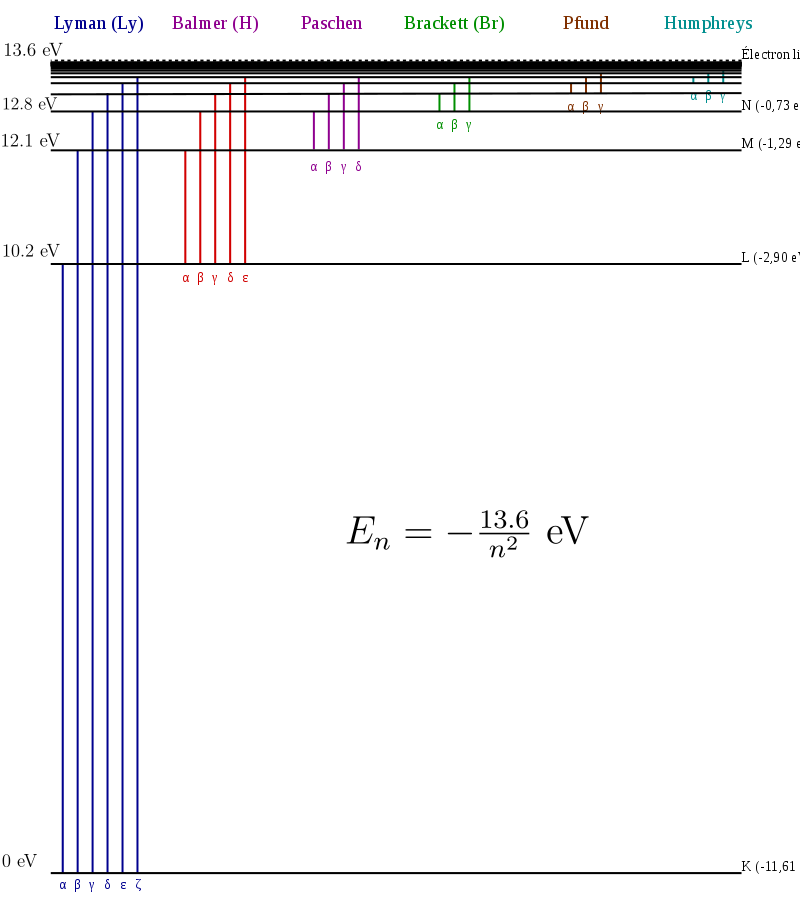
\includegraphics[width=0.5\textwidth]{figures/serie_idrogeno.png}
	\caption{\scriptsize Serie spettrale dell'idrogeno}
	\label{fig:-figures-serie_idrogeno-png}
\end{figure}
I livelli dell'atomo di idrogeno prendono la forma della Figura \ref{fig:-figures-serie_idrogeno-png}, possiamo notare diverse serie di energie che descrivono i livelli, ognuna avente il suo nome caratteristico.\\
Se mettiamo per comodità lo zero dell'energia sullo stato fondamentale abbiamo che i livelli energetici seguono la serie scritta in Figura \ref{fig:-figures-serie_idrogeno-png}.\\
Immaginiamo di voler far avvenire una transizione energetica dell'elettrone nell'idrogeno, a seconda del livello di partenza l'energia necessaria seguirà una determinata serie:
\begin{align}
	n=1 \ \to \ m \ge 2 \ &\implies \ \text{ Assorbimento da Lyman}\\
	n=2 \ \to m\ge 3 \ &\implies \ \text{ Assorbimento da Balmer} \\
			   &\ldots
.\end{align}
Il passaggio invece "dall'alto al basso" sarà l'emissione nelle varie serie.\\ 
Per la Lyman $\alpha $ ad esempio si ha che, se si emette o si assorbe un fotone dal primo stato eccitato al fondamentale (o viceversa) si ha che:
\begin{align}
	&\ce{n = 1 <-> n = 2 }  & E_{L_{\gamma \alpha }} = 10.2 \text{ eV}& &\lambda = 1216 \text{\AA}
.\end{align}
Mentre per la Lymann $\beta $:
\begin{align}
	&\ce{n = 1 <-> n = 3 }  & E_{L_{\gamma \beta  }} = 12.1 \text{ eV}& &\lambda = 1020 \text{\AA}
.\end{align}
E così via fino al salto di Lymann
\begin{align}
	&\ce{n = 1 <-> n = \infty }  & E_{L_{\infty}} = 13.6 \text{ eV}& &\lambda = 912 \text{\AA}
.\end{align}
Vediamo che questa serie è tutta nell'ultravioletto, questo è importante e dobbiamo tenerlo a mente.\\
Un'altra serie importante è la Balmer:
\begin{align}
	&\ce{n = 2 <-> n = 3 }  & E_{H_{\alpha }} = 1.9 \text{ eV}& &\lambda = 6563 \text{\AA}
.\end{align}
E così via fino al salto di Balmer:
\begin{align}
	&\ce{n = 2 <-> n = \infty }  & E_{H_{\infty }} = 3.5 \text{ eV}& &\lambda = 3646 \text{\AA}
.\end{align}
È utile notare che la serie di Balmer parte dal rosso e arriva all'ultravioletto con il salto, quindi gran parte della serie sta nel visibile, quindi quelle di Balmer sono le righe che possiamo vedere tecnicamente anche ad occhio nudo.
\subsection{Radiazione attraverso una nube interstellare}%
Ipotizziamo che il mezzo sia una nube di mezzo interstellare composta da idrogeno. La temperatura della nube è quella tipica di queste nubi: $T \approx 100$ K. Spariamo sulla nube due fasci aventi energie diverse:
\begin{align}
	&L_{\gamma,\alpha} \\
	&H_{\alpha}
.\end{align}
Ci chiediamo adesso se la nube sarà trasparente oppure opaca ai fasci inviati.\\
Se l'atomo di idrogeno si trova nello stato fondamentale allora il fotone dell'$H_{\alpha}$ non può essere assorbito, non ha l'energia per fare il salto, quindi tutti gli atomi di idrogeno sono invisibili per un fotone della $H_{\alpha}$. \\
Il fotone della $L_{\gamma,\alpha}$ invece ha l'esatta energia per effettuare il salto, quindi viene assorbito. \\
È quindi è importante capire se ci sono e quanti sono gli atomi nel primo eccitato, perchè se ci sono allora $H_{\alpha}$ viene assorbito avente l'esatta energia per permettere il salto. \\
Per capire se $H_{\alpha }$ viene assorito dalla nube è necessario capire in che stato si trovano gli atomi della nube.\\
Procediamo quindi assumendo che la nube sia all'equilibrio termodinamico e cerchiamo il rapporto tra gli atomi del primo eccitato e quello fondamentale con la distribuzione di Boltzmann:
\[
	\frac{n_2}{n_1} = \frac{g_2}{g_1}\exp\left( -\frac{\Delta E_{1,2}}{kT} \right) 
.\] 
Le $g$ sono le degenerazioni dell'atomo di idrogeno (i pesi statistici): $g_{n}= 2 n^2$ mentre $n_2$ è il numero di atomi di idrogeno che si trovano nel primo eccitato, $n_1$ è il numero di quelli che si trovano nel fondamentale. \\
Abbiamo che $ \ g_2 = 8 \ $, $ \ g_1 = 2 \ $,  $ \ \Delta E _{1,2}= 10.2 \ $eV, $ \ kT =\frac{1}{120} \ $ eV \footnote{Per ricordare questa si può ricordare che a temperatura ambiente kT = $\frac{1}{40}$ eV, quindi si ricava anche alla nostra temperatura. Sulla superficie del sole, con temperature dell'ordine di 6000 K, sarà circa mezzo eV (emissione nel visibile). Nel centro del sole invece, con circa 16 milioni di K, si ha $kT \approx$ 1 keV (emissione nell'X).}.\\
\[
	\frac{n_2}{n_1} = 4 \exp\left( - \frac{10.2}{1 / 120} \right)  = 4 \exp\left( -1224 \right) = 4\cdot 10^{-1224 /2.3} \approx 10^{-532}
.\] 
Dove abbiamo usato il fattore di conversione tra esponenziali nelle due basi.\\
Abbiamo un atomo nell'eccitato ogni $10^{532}$ atomi nel fondamentale. Bisonga capire quanti atomi ha la nube per dire se il numero di atomi che si trovano effettivamente nel primo eccitato non è trascurabile. \\
Per risolvere la questione basta però notare che $10^{532}$ sono troppi atomi persino per l'universo stesso!
\paragraph{Stima del numero di atomi nell'universo}%
La massa del sole è $2 \cdot 10^{33} $ g, la massa dell'idrogeno $M_{H} = 1.66 \cdot 10^{-24}$ g quindi il numero di atomi nel sole sarà dell'ordine di $n_{_{\odot}} = 10^{57}$, nella galassia ci sono circa $10^{11}$ stelle, quindi il numero di particelle idrogenoidi nella galassia potrebbe essere dell'ordine di $n_{\text{galassia}} \approx 10^{68}$. 
Visto che ci sono nell'universo visibile abbiamo circa $10^{11}$ galassie, quindi in tutto nell'universo visibile possiamo stimare circa $n_{\text{universo}} \approx 10^{80}$ atomi. 
Un numero incredibiblmente più piccolo di quello trovato da noi sopra.\\
Tornando all'esercizio possiamo stare molto tranquilli sul fatto che nella nube non ci saranno idrogeni nel primo eccitato, saranno tutti nel fondamentale, quindi la nube è otticamente sottile al fascio $H_{\alpha}$ anche se fosse estesa per milioni di chilometri.\\
Viceversa i fotoni della $L_{\alpha }$ verranno assorbiti, la nube sarà opaca a questi fotoni.\\
Questo ci anticipa anche che se in un mezzo come quello sopra gli atomi si eccitano (tipicamente per collisioni) e si diseccitano successivamente nella $H_{\alpha }$ allora i fotoni emessi usciranno dal mezzo indisturbati portando con se dell'energia. 
Questo è una tecnica di raffreddamento per il mezzo stesso che può perdere energia per collisioni e successiva emissione.\\
Inoltre se andiamo sul sito dell'hubble space telescope e cerchiamo le regioni di formazione stellare $H_2$ vediamo delle regioni di un colore rossastro, questo è proprio $H_{\alpha }$ che, con i suoi $6563$ \AA $ \ $  esce dalla nube per arrivare alla lente di Hubble.
\begin{figure}[H]
	\centering
	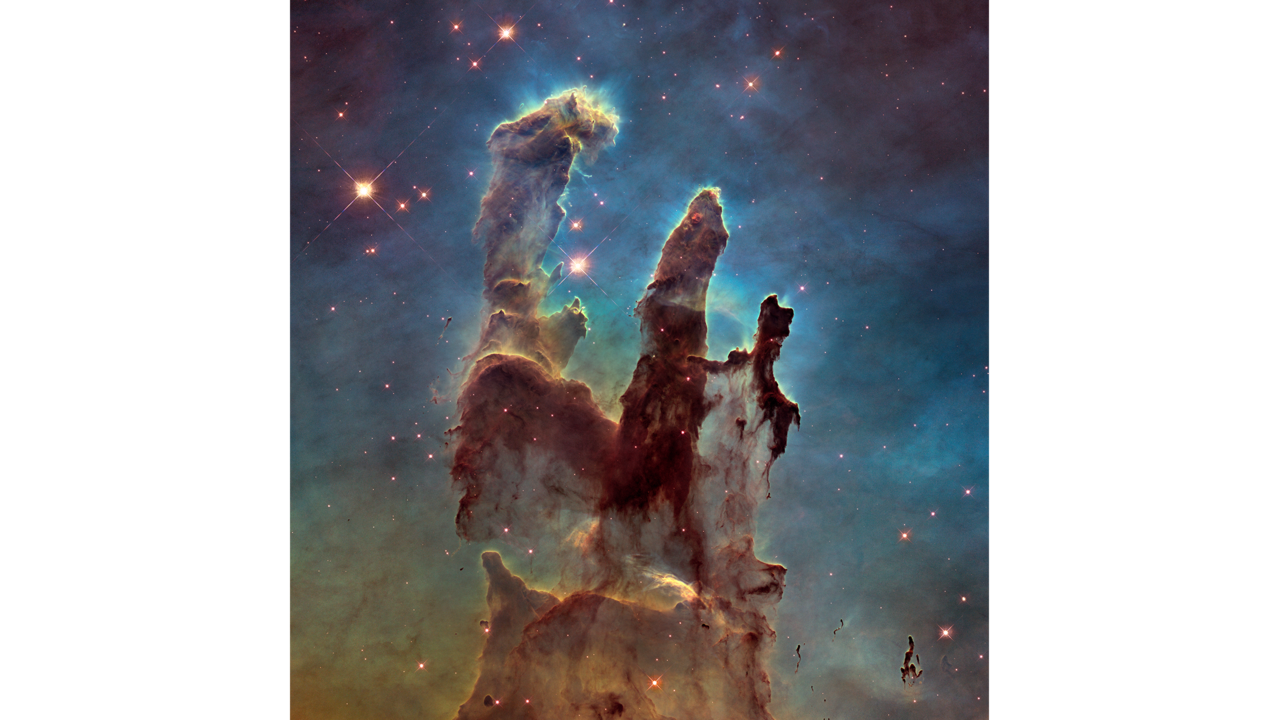
\includegraphics[width=0.8\textwidth]{figures/veil-nebula.png}
	\caption{\scriptsize Immagine di una nebulosa nel visibile (modificata per accentuare la nitidezza).}
	\label{fig:figures-veil-nebula-png}
\end{figure}
\noindent
\subsection{Soluzione analitica all'equazione del trasporto stazionaria.}%
Abbiamo visto che l'espressione dell'equazione del trasporto in condizioni stazionarie si riduce a:
\[
	\frac{\mbox{d} I_{\nu}}{\mbox{d} s} = j _{\nu} - \alpha_{\nu}I_{\nu} 
.\] 
Vogliamo fare un cambio di variabile, anzichè studiarla rispetto alla variabile $s$ la vogliamo rispetto alla profondità ottica $\tau _{\nu} $.
\[
	\frac{\mbox{d} I_{\nu}}{\mbox{d} s} = \frac{\mbox{d} I_{\nu}}{\mbox{d} \tau_{\nu}} \frac{\mbox{d} \tau_{\nu}}{\mbox{d} s} = \frac{\mbox{d} I_{\nu}}{\mbox{d} \tau_{\nu}} \alpha_{\nu} = j _{\nu} - \alpha_{\nu}I_{\nu}
.\]
L'equazione modificata diventa:
\[
	\frac{\mbox{d} I_{\nu}}{\mbox{d} \tau_{\nu}}  = \frac{j _{\nu}}{\alpha_{\nu}}- I_{\nu}
.\] 
Possiamo allora definire il primo termine dopo l'uguale come:
\begin{defn}[Funzione sorgente]{def:Funzione sorgente}
	Il rapporto tra il coefficiente di emissione ed il coefficiente di assorbimento è detto funzione sorgente $s_{\nu} $:
	\[
		s_{\nu} = \frac{j _{\nu} }{\alpha _{\nu} }
	.\] 
\end{defn}
L'equazione del trasporto con questo termine è ovviamente:
\[
	\frac{\mbox{d} I_{\nu}}{\mbox{d} \tau_{\nu}} = s_{\nu}- I_{\nu}
.\] 
Possiamo notare inoltre che 
\[
s_{\nu}<I_{\nu} \implies \frac{\mbox{d} I_{\nu}}{\mbox{d} \tau_{\nu}} <0
.\]
In questo modo l'intensità del fascio viene attenuata nell'attraversare la nube. Viceversa:
\[
s_{\nu}>I_{\nu} \implies \frac{\mbox{d} I_{\nu}}{\mbox{d} \tau_{\nu}} >0
.\]
Quindi il fascio viene amplificato nel passagio.\\
Proviamo a risolvere formalmente l'equazione:
\[
	\frac{\mbox{d} I_{\nu}}{\mbox{d} \tau_{\nu}}e^{\tau_{\nu}} = s_{\nu}e^{\tau_{\nu}}- I_{\nu}e^{\tau_{\nu}}
.\] 
Quindi possiamo raggruppare:
\[
	\frac{\mbox{d} }{\mbox{d} \tau _{\nu} } \left( I_{\nu}e^{\tau_{\nu}} \right) = s_{\nu}e^{\tau_{\nu}}
.\] 
e integriamo tra 0 e $\tau _{\nu} $:
\[
	\int_{0}^{\tau_{\nu}}\frac{\mbox{d} }{\mbox{d} \tau'_{\nu}} \left( I_{\tau'_{\nu} } e^{\tau' _{\nu} } \right) d\tau '_{\nu}  = 
	\int_{0}^{\tau _{\nu} } s( \tau '_{\nu} ) e^{\tau '_{\nu} }d\tau _{\nu} 
.\] 
integrando il primo termine ottiene: 
\[
	I_{\nu}\left( \tau_{\nu} \right) e^{\tau_{\nu}} - I_{\nu}\left( 0 \right) = 
	\int_{0}^{\tau_{\nu}} s_{\nu}\left( \tau_{\nu}' \right) e^{\tau_{\nu}'}d \tau_{\nu}'
.\] 
Se dividiamo tutto per $e^{\tau _{\nu} }$ abbiamo la legge per $I_{\nu} ( \tau _{\nu} ) $.
\begin{fact}[Soluzione formale all'equazione del trasporto]{fact:Soluzione formale all'equazione del trasporto}
	\[
	I_{\nu}\left( \tau_{\nu} \right) = I_{\nu}\left( 0 \right)e^{-\tau_{\nu}} - \int_{0}^{\tau_{\nu}} \delta_{\nu}\left( \tau_{\nu}' \right) e^{-(\tau_{\nu}-\tau_{\nu}')}d \tau_{\nu}'
.\] 
\end{fact}
Il primo termine è la luce della sorgente estinta esponenzialmente dal mezzo a causa dell'assorbimento. Il secondo termine contiene il significato fisico di due distinti effetti: l'effetto dell'emissione di fotoni del fascio nei vari punti del mezzo ($s_{\nu} $) e l'effetto dell'assorbimento incluso nel termine esponenziale.\\
Innfatti il termine $\tau _{\nu} -\tau '_{\nu} $ sta ad indicare l'assorbimento dei fotoni che sono stati emessi dal mezzo. \\
Anche se abbiamo la soluzione generale resta il fatto che $s_{\nu} $ è incognita, anche se conoscessimo l'espressione analitica di $s_{\nu} $ non saremo comunque in grado di calcolare l'integrale poichè non conosciamo le condizioni fisiche (pressione, temperatura \ldots) del mezzo \footnote{dalle quali ricordiamo dipendere $\tau _{\nu} $}.
\paragraph{Esempio: mezzo omogeneo.}%
Se il mezzo è omogeneo per tutta la sua estensione si mantengono costanti le sue proprietà fisiche. Di conseguenza avremo che $\alpha _{\nu} $ e $j _{\nu} $ saranno uguali ovunque e la funzione sorgente sarà anch'essa una costante:
\[
	I_{\nu}\left( \tau_{\nu} \right) = I_{\nu}\left( 0 \right) e^{-\tau_{\nu}} + s_{\nu} e^{-\tau_{\nu}}\int_0^{\tau_{\nu}} e^{\tau_{\nu}'}d \tau_{\nu}' =
	I_{\nu}\left( 0 \right) e^{-\tau_{\nu}} + s_{\nu}\left( 1-e^{-\tau_{\nu}} \right) \label{eq:soluzione-mezzo-omogeneo}
.\] 
Possiamo iniziare ad intuire il significato fisico della funzione sorgente:
se il nostro fascio attraversa un mezzo otticamente profondo ($\tau_{\nu}\rightarrow \infty$) allora abbiamo che $I_{\nu}\left( \tau_{\nu} \right) \rightarrow s_{\nu}$. Allora la funzione sorgente è la grandezza fisica a cui tende l'intensità della radiazione se questa attraversa una regione otticamente spessa. Quindi ciò che succede al fascio in questo caso è una totale sostituzione dei fotoni provenienti dalla sorgente con i fotoni emessi all'interno del mezzo come in Figura \ref{fig:soluzione-all-equazione-del-trasporto-per-mezzo-otticamente-spesso}
\begin{figure}[H]
    %This is a custom LaTeX template!
    \centering
    \incfig{soluzione-all-equazione-del-trasporto-per-mezzo-otticamente-spesso}
    \caption{\scriptsize Sostituzione dei fotoni in un mezzo otticamente spesso.}
    \label{fig:soluzione-all-equazione-del-trasporto-per-mezzo-otticamente-spesso}
\end{figure}
\noindent
Man mano che la radiazione si propaga i fotoni del fascio perderanno le caratteristiche della radiazione sorgente ed acquisteranno invece la firma del mezzo.\\
Notiamo che questo non è soltanto un processo astrofisico, questo avviene anche quando guardiamo delle montagne lontane che ci appaiono celestine come il cielo:
\begin{figure}[H]
	\centering
	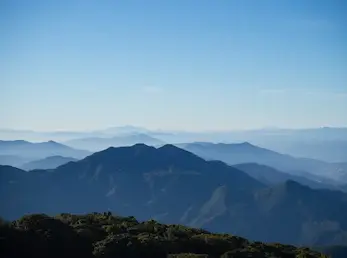
\includegraphics[width=0.4\textwidth]{figures/farmountain.png}
	\caption{\scriptsize Montagne lontane che acquistano il colore del cielo fino a dissolversi con esso.}
	\label{fig:figures-farmountain-jpg}
\end{figure}

\paragraph{Esempio: Mezzo omogeneo senza retroilluminazione}
In questo caso particolare abbiamo che $I_{\nu} ( 0) = 0$, l'unica radiazione che vediamo emergere è quella prodotta dal mezzo stesso.
\[
	I_{\nu} ( \tau _{\nu} ) = s_{\nu}\left( 1-e^{-\tau _{\nu} } \right)  
.\] 
Consideriamo adesso i casi in cui il mezzo è otticamene sottile o spesso alla radiazione che emerge da lui stesso.
\subparagraph{Mezzo otticamente sottile}
Siamo in questa situazione se $\tau _{\nu} \ll 1$, sviluppiamo l'esponenziale:
\[
	I_{\nu} ( \tau _{\nu} ) = s_{\nu} \tau _{\nu} 
.\] 
Visto che il mezzo è omogeneo si ha:
\[
	\tau _{\nu} = \int_{s_0}^{s} \alpha _{\nu} ( s') ds'= \alpha _{\nu} ( s-s_0)  = \alpha _{\nu} \cdot L
.\] 
Quindi abbiamo che:
\[
	I_{\nu} ( \tau _{\nu} ) = s_{\nu} \alpha _{\nu}\cdot  L = j _{\nu} \cdot L
.\] 
Dalla quale emerge l'importante contributo alla radiazione di $j _{\nu} $ in questa situazione.\\
Se il mezzo è costituito da atomi non completamente ionizzati allora sappiamo che la radiazione ha dei picchi in intensità molto marcati in corrispondenza della frequenza di transizione dei livelli, quindi sia il coefficiente di assorbimento $\alpha _{\nu} $ che il coefficiente di emissione $j _{\nu} $ avranno dei picchi molto marcati in corrispondenza di queste transizioni. Quindi qua ci aspettiamo proprio questo tipo di radiazione proveniente dal "mezzo", molto marcata in corrispondenza della transizione dei livelli delle specie atomiche. \\
Questa radiazione emergente sarà perciò caratterizzato da delle righe di emissione: uno spettro buio quasi ovunque con delle righe luminose.\\
Un esempio di questo tipo è un gas rarefatto riscaldato: una lampada al neon. Un esempio nello spazio sono le nebulose. \footnote{Nelle stelle invece vedo delle righe di assorbimento miste al continuo}
\subparagraph{Mezzo otticamente spesso}
Quando scaldiamo un oggetto a temperature elevate inizia ad essere percepibile la sua emissione di radiazione termica, questo passerà in modo continuo dal rosso scuro, poi al giallo, ecc\ldots \\
Prendiamo un mezzo omogeneo non retroilluminato ed otticamente spesso $\tau _{\nu} \gg 1$, in questo limite abbiamo che:
\[
	I_{\nu} ( \tau _{\nu} )  = s_{\nu} 
.\] 
Quindi la radiazione che emerge è uguale alla funzione sorgente, questo è il caso del oggetto riscaldato. Infatti la funzione sorgente è parente della radiazione di corpo nero che è una funzione della temperatura. Quindi in questo caso abbiamo uno spettro continuo.\\
Nel cosmo oggetti che approssimeranno questa radiazione sono le stelle, non sara esattamente una radiazione di corpo nero perchè abbiamo delle righe di assorbimento. Studieremo prossimamente da dove vengono queste misteriose righe di assorbimento.

\lez{4}{02-03-2020}{}
\[
	\frac{\mbox{d} I_{\nu} }{\mbox{d} s} = j _{\nu} -\alpha _{\nu} \quad d\tau _{\nu} = \alpha _{\nu} ds \text{ Profondità ottica}
.\] 
\[
	\frac{\mbox{d} I_{\nu} }{\mbox{d} \tau _{\nu} } = s_{\nu} - I_{\nu} \quad S_{\nu} = \frac{j _{\nu} }{\alpha _{\nu} } \text{S: funzione sorgente}
.\] 
Soluzione formale eq. trasporto
\[
	I_{\nu} ( \tau _{\nu} ) = I_{\nu} ( 0) e^{-\tau _{\nu} } + \int_{0}^{\infty} s_{\nu} ( \tau _{\nu} ) e^{-\left( \tau _{\nu} -\tau _{\nu} ' \right) }
	\text{ messo omogeneo}
.\] 
Caso di mezzo omogeneo:
\[
	I_{\nu} ( \tau _{\nu} ) = I_{\nu} ( 0) e^{-\tau _{\nu} } + S_{\nu} \left( 1- e^{-\tau _{\nu} } \right) 
.\] 
\[
	\text{Se } \tau _{\nu} \gg 1 \implies I_{\nu} ( \tau _{\nu} ) \to S_{\nu} 
.\] 
Altrimenti
\[
	I_{\nu} ( \tau _{\nu} )  \approx j _{\nu} L
.\] 
\subsection{Scoperta delle righe}%
Le righe sono state scoperte osservando lo spettro del sole, 



\end{document}
